\input /users/davidmcallester/icloud/tex/SlidePreamble
\input /users/davidmcallester/icloud/tex/preamble

\begin{document}

{\Huge

  \centerline{\bf TTIC 31230, Fundamentals of Deep Learning}

\bigskip

\centerline{David McAllester, Autumn  2024}

\vfill \vfill

\centerline{\bf Variational Auto-Encoders (VAEs)}

\vfill \vfill

\slide{Fundamental Equations of Deep Learning}

\begin{itemize}
\item Cross Entropy Loss: $\Phi^* = {\color{red} \argmin_\Phi E_{(x,y)\sim \pop}\left[-\ln P_\Phi(y|x)\right]}$.

\vfill
\item GAN: $\gen^* = {\color{red} \argmax_{\gen} \min_{\disc} E_{i \sim \{-1,1\}, y \sim P_i}\left[-\ln P_{\disc}(i|y)\right]}$.

\vfill
\item VAE (including diffusion models)
\begin{eqnarray*}
& & \pri^*,\dec^*,\enc^* \\
\\
& = & {\color{red} \argmin_{\pri,\dec,\enc}\;E_{y \sim \pop,z \sim P_\enc(z|y)}\left[ - \ln \frac{P_\pri(z)P_\dec(y|z)}{P_\enc(z|y)}\right]}
\end{eqnarray*}
\end{itemize}

\slide{VAEs}
A variational autoencoder (VAE) is defined by three parts:

\vfill
\begin{itemize}
\item An encoder distribution $P_\enc(z|y)$.

\vfill
\item A ``prior'' distribution $P_\pri(z)$

\vfill
\item A generator distribution $P_\dec(y|z)$
\end{itemize}

\vfill
VAE generation uses $P_\pri(z)$ and $P_\dec(y|z)$ (like a GAN).

\vfill
VAE training uses an encoder $P_\enc(z|y)$.

\slide{Fixing an Arbitray Encoder}
Fix the encoder arbitrarily and train $P_\pri$ and $P_\dec$ by cross entropy loss.

$${\color{red}\pri^*,\dec^* = \argmin_{\pri,\dec}\;E_{y \sim \pop(y),z \sim \enc(z|y)}\left[-\ln P_\pri(z)P_\dec(y|z)\right]}$$

\vfill
Universality gives

{\color{red} $$P_{\pri^*}(z)P_{\dec^*}(y|z) = \pop(y)P_\enc(z|y)$$}

\vfill
Sampling from $P_{\pri^*}(z)P_{\dec^*}(y|z)$ now samples $y$ from the population.

\slide{Training the Encoder --- the ELBO}

In practice the choice of encoder matters.

\begin{eqnarray*}
P(y) & = & \frac{\pop(y)P_\enc(z|y)}{P_\enc(z|y)} \;=\; \frac{P_\enc(z)P_\enc(y|z)}{P_\enc(z|y)} \\ \\
\\
H(y) & \leq & E_{y \sim \pop,z \sim P_\enc(z|y)}\left[ - \ln \frac{P_\pri(z)P_\dec(y|z)}{P_\enc(z|y)}\right]
\end{eqnarray*}

\vfill
The inequality follows from the fact that cross-entropy (using the models $P_\pri$ and $P_\dec$) upper bounds entropy.

\vfill
This upper bound on $H(y)$ is called {\bf the ELBO} (Acronym described later).

\slide{Difficulties in Training the Encoder}


$$\enc^* = \argmin_{\enc}\;\;E_{y\sim \pop(y),{\color{red} z\sim P_\enc(z|y)}}\;\left[- \ln \frac{P_\pri(z)P_\dec(y|z)}{{\color{red} P_\enc(z|y)}}\right]$$

\vfill
Gradient descent on the encoder parameters must take into account the fact that we are sampling from the encoder.

\vfill
Training a sampling distribution typically suffers from mode collapse (as in GANs).

\vfill
Often the encoder collapses to fixing $z = 0$. $P_\dec(y|z)$ can always just ignore $z$. We are then back to standard cross-entropy loss.
This is called posterior collapse.

\slide{Types of VAEs}

In {\bf a Gaussian VAE} the we have $P_\pri(z)$ and $P_\enc(z|y)$ are both Gaussian distributions on $R^d$.
A diffusion model involves a Gaussian VAE at each incremental step of diffusion.

\vfill
{\bf A Vector Quantized VAE} (VQ-VAE) defines $P\enc(z|y)$ in terms of vector quantization analogous to $K$-means clustering.
VQ-VAEs provide a translation from continuous data, such as images, to token data that can be modeled with a transformer.
This is done in Chat-GPT 4o and other multi-modal language models.

\vfill
We will consider each these approaches.

\slide{Gaussian VAEs}


\vfill
We sample noise $\epsilon$ from a Gaussian distribution on $R^d$.

\vfill
{\huge
\begin{eqnarray*}
\enc^* & = & \argmin_{\enc}\;\;E_{y,{\color{red} \epsilon \sim {\cal N}(0,\sigma I)}}\;\left[- \ln \frac{P_\pri(z)P_\dec(y|z)}{P_\enc(z|y)}\right]\;\;z = \hat{z}(y) + \epsilon \\
\\
\\
& = & \argmin_\enc\;{\color{red} KL(P_\enc(z|y),P_\pri(z))} + E_{z \sim P_\enc(z|y)}\left[- \ln P_\dec(y|z)\right] \\
\\
\\
&=& \argmin_\enc\;{\color{red} \frac{||\hat{z}_\enc(y) - \hat{z}_\pri||^2}{2\sigma^2}} + E_\epsilon\;\frac{||y - \hat{y}_\dec(\hat{z}_\enc(y,\epsilon))||^2}{2\sigma^2}
\end{eqnarray*}


\vfill
A closed-form expression for the KL term avoids sampling noise.
}

\slide{VAEs Evolved from Variational Bayesian Inference}

$P_\pri(z)$ is interpreted as the Bayesian prior on ``hypothesis'' $z$.

\vfill
$P_\dec(y|z)$ is interpreted as the propability of the ``evidence'' $y$ given hypothesis $z$.

\vfill
We consider the Bayesian distribution defined by $P_\pri(z)$ and $P_\dec(y|z)$ and we want to compute $P_{\pri,\dec}(z|y)$
under this Bayesian distribution.  I will write this $P_{\mathrm{Bayes}}(z|y)$

\vfill
$P_\enc(z|y)$ is interpreted as an approximation for $P_{\pri,\dec}(z|y)$.

\slide{Bayesian Interpretation}
{\huge
\begin{eqnarray*}
\ln P_{\mathrm{Bayes}}(y) & =  & \ln \frac{P_{\mathrm{Bayes}}(y)(z)P_{\mathrm{Bayes}}(z|y)}{P_{\mathrm{Bayes}}(z|y)} \\
\\
\\
& = & E_{z \sim P_\enc(z|y)} \left[\ln \frac{P_{\pri}(z)P_\dec(y|z)}{P_{\mathrm{Bayes}}(z|y)}\right] \\
\\
\\
& \geq & E_{z \sim P_\enc(z|y)}\left[\ln \frac{P_{\pri}(z)P_\dec(y|z)}{P_\enc(z|y)}\right] \\
\end{eqnarray*}
}
Here we have replaced a cross-entropy by an entropy.

\slide{Bayesian Interpretation}
{\huge
\begin{eqnarray*}
\ln P_{\mathrm{Bayes}}(y) & \geq & E_{z \sim P_\enc(z|y)}\left[\ln \frac{P_{\pri}(z)P_\dec(y|z)}{P_\enc(z|y)}\right] \\
\end{eqnarray*}
}

Here $y$ is the evidence about $z$ under the Bayesian model.

\vfill
This is the {\bf evidence lower bound} or {\bf ELBO}.

\slideplain{Expectation Maximization (EM)}

Expectation Maximimization (EM) applies in the (highly special) case where the exact posterior $P_{\pri,\dec}(z|y)$ is samplable and computable.
EM alternates exact optimization of $\enc$ and the pair $(\pri,\dec)$ in:
$$\mbox{VAE:}\;\;\;\;\;\;\; {\color{red} \pri^*,\dec^*} = \argmin_{\color{red} \pri,\dec} \min_{\color{red} \enc} E_{y,\;z \sim P_{\color{red} \enc}(z|y)}\;\;- \ln \frac{P_{\color{red} \pri,\dec}(z,y)}{P_{\color{red} \enc}(z|y)}$$

\vfill
$$\mbox{EM:}\;\;\;\;\;\; {\color{red} \pri^{t+1},\dec^{t+1}} =  \argmin_{\color{red} \pri,\dec}\;\;\;\;E_{y,\;z \sim P_{\color{red} \pri^t,\dec^t}(z|y)}\; - \ln P_{\color{red} \pri,\dec}(z,y)$$

\vfill
\centerline{\hspace{1em} Inference \hspace{6em} Update \hspace{2.5em}~}
\centerline{(E Step) \hspace{6em} (M Step) ~}
\centerline{ $P_\enc(z|y) = P_{\pri^{\color{red} t},\dec^{\color{red} t}}(z|y)$ \hspace{2.5em} Hold $P_\enc(z|y)$ fixed \hspace{0em}~}
\
slide{Posterior Collapse}


{\color{red} $$P_\pri(z)P_\dec(y|z) = \pop(y)P_\enc(z|y)$$}

\vfill
Any joint distribution on $(y,z)$ with the desired marginal on $y$ optimizes the bound.

\vfill
This allows the prior and the encoder (the posterior) to both degenerate to having no mutual information with $y$.

\vfill
This often happens in language modeling.

\slide{Hierarchical VAEs}


\centerline{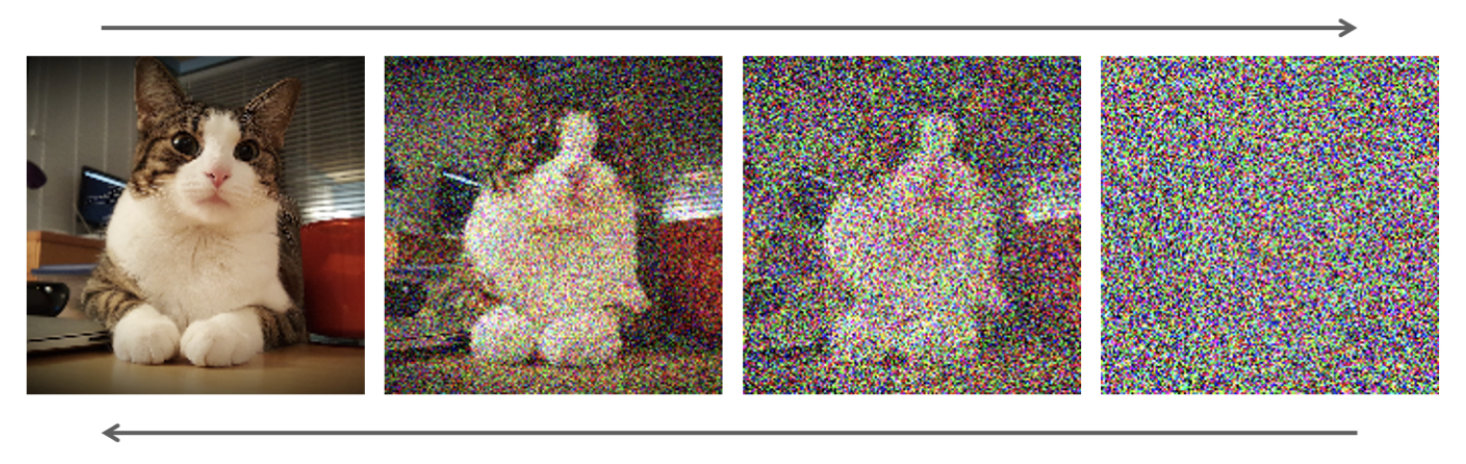
\includegraphics[width = 7in]{\images/DiffSequence}}

\vfill
{\huge
\centerline{{\color{red} [Sally talked to John]} $\stackrel{\rightarrow}{\leftarrow}$ {\color{red} [Sally talked to]}
$\stackrel{\rightarrow}{\leftarrow}$ {\color{red}[Sally talked]} $\stackrel{\rightarrow}{\leftarrow}$ {\color{red}[Sally]} $\stackrel{\rightarrow}{\leftarrow}$ {\color{red} []}}
}

\vfill
\centerline{$y \stackrel{\rightarrow}{\leftarrow} z_1  \stackrel{\rightarrow}{\leftarrow} \cdots \stackrel{\rightarrow}{\leftarrow} z_N$}

\slide{Hierarchical VAEs}
\centerline{$y \stackrel{\rightarrow}{\leftarrow} z_1  \stackrel{\rightarrow}{\leftarrow} \cdots \stackrel{\rightarrow}{\leftarrow} z_N$}

\vfill
{\bf Encoder}: $\pop(y)$, $P_\enc(z_1|y)$, and $P_\enc(z_{\ell+1}|z_\ell)$.


\vfill
{\bf Generator}: $P_\pri(z_N)$, $P_\dec(z_{\ell-1}|z_\ell)$, $P_\dec(y|z_1)$.

\vfill
The encoder and the decoder define distributions $P_\enc(y,\ldots,z_N)$ and $P_\dec(y,\ldots,z_N)$ respectively.


\slide{Hierarchical VAEs}

\centerline{$y \stackrel{\rightarrow}{\leftarrow} z_1  \stackrel{\rightarrow}{\leftarrow} \cdots \stackrel{\rightarrow}{\leftarrow} z_N$}

\vfill
\begin{itemize}
\item autoregressive models

\vfill
\item diffusion models
\end{itemize}


\slide{Hierarchical (or Diffusion) ELBO}

{\Large
\begin{eqnarray*}
H(y) & = & E_\enc\left[- \ln\frac{P_\enc(y)P_\enc(z_1,\ldots,z_N|y)}{P_\enc(z_1,\ldots,z_N|y)}\right]\\
  \\
  \\
  & = & E_\enc\left[ - \ln\frac{P_{\color{red} \enc}(y|z_1)P_{\color{red} \enc}(z_1|z_2)\cdots P_{\color{red} \enc}(z_{N-1}|z_N)P_{\color{red} \enc}(z_N)}
  {P_\enc(z_1|z_2,y)\cdots P_\enc(z_{N-1}|z_N,y)P_\enc(z_N|y)}\right] \\
   \\
   \\
  & {\color{red} \leq} & E_\enc\left[ - \ln\frac{P_{\color{red} \dec}(y|z_1)P_{\color{red} \dec}(z_1|z_2)\cdots P_{\color{red} \dec}(z_{N-1}|z_N)P_{\color{red} \dec}(z_N)}
  {P_\enc(z_1|z_2,y)\cdots P_\enc(z_{N-1}|z_N,y)P_\enc(z_N|y)}\right] \\
\\
\\
 & = & \left\{\begin{array}{l}E_\enc\;[-\ln P_\dec(y|z_1)]
                             \\ \\ + \sum_{i=2}^N  \; E_\enc\; KL(P_\enc(z_{i-1}|z_i,y),\;P_\dec(z_{i-1}|z_i)) \\
                             \\ + E_\enc\; KL(P_\enc(Z_N|y),p_\dec(Z_N))\end{array}\right.
\end{eqnarray*}
}

\slide{END}

\end{document}
